\section{Fiche de bilan et de synthèse}
\subsection{Présentation de l'activité en entreprise}
\subsubsection{L'entreprise d'accueil}
L’entreprise Kappa Santé a été créée en 2003 par Mr SCHÜCK (médecin de
santé publique) et par Mme TEXIER (pharmacienne) en vue d’apporter des
services de qualité. Avec une expertise ciblée sur les domaines de:
l’épidémiologie, pharmaco- épidémiologie, la constitution d’e-cohortes i et des
interventions en santé publique et numérique, cette société répond aux
demandes à la fois au niveau national et européenne.
Cette CRO (Contract Research Organization) est une SAS (Société Anonyme
Simplifiée) au capital de 50 000 €.
Le siège social de l’entreprise est situé au 4 rue Cléry à Paris, dans le 2e
arrondissement.
Kappa Santé est membre de l’ENCEPP (European Network of Centres for
Pharmacoepidemiology and Pharmacovigilence), de l’AFCROs (association de
CRO) et du pôle compétitivité numérique Cap digital (collectif européen
d’innovateurs).
L’entreprise Kappa Santé est l’entreprise mère de Kap Code depuis 2015. Kap
Code est une entreprise qui récupère des données liées à la santé sur les
réseaux sociaux.
En mars 2023, Kappa Santé a été racheté par Apices, une entreprise CRO
espagnole qui réalise des études cliniques.
À ses débuts, Kappa Santé réalisait des études dans le but de recueillir des
informations sur des médicaments mais depuis 2012, la société s’est diversifiée
et est devenue polyvalente en proposant des services comme le suivi et le
monitoring, la création de protocole, ...
De grosses entreprises comme Pfizer, Janssen, AstraZeneca, Microsoft, IBM... font confiance à Kappa Santé. Les principaux concurrents de Kappa Santé sont
Aixial, Axonal, Cemka, Clinact, Euraxi, Icon, Icta, Iqvia, Sanoïa...

L’équipe dont je fais partie intègre le Département Informatique où M. BRUNAT est le directeur informatique.

\begin{figure}[H]
    \centering
    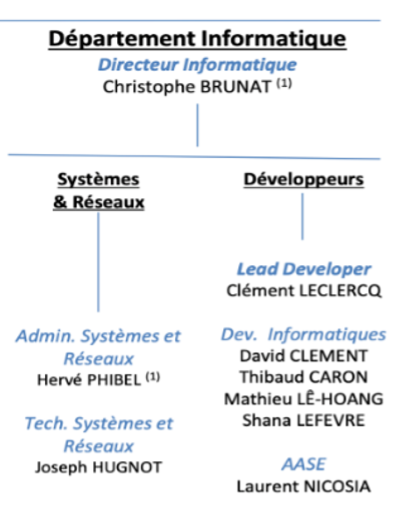
\includegraphics[width=0.4\textwidth]{fiche_bilan/fiche_bilan_images/organigramme_info.png} 
    \caption{Organigramme de l'entreprise}
\end{figure}
Nous développons en Java à l’aide du Framework JSF (Java Server Faces) et
des composants PrimeFaces.
Pour communiquer avec notre base de données (développeur), JPA définit des
entités qui sont une instance de classe et nous permet d’écrire des
programmes qui interagissent avec la base de données.
\begin{figure}[H]
    \centering
    \includegraphics[width=0.3\textwidth]{fiche_bilan/fiche_bilan_images/intégration_jpa.png} 
    \caption{Schéma d'intégration de JPA}
\end{figure}

\subsubsection{Le maître d'apprentissage}
Notre équipe est composée de cinq développeurs, encadrés par un « lead developer », Monsieur Clément LECLERCQ (voir schéma précédent), qui assure le rôle de superviseur. Il prend les décisions stratégiques, coordonne les projets, organise et anime des réunions afin de représenter l’équipe des développeurs. Il est également mon maître d’apprentissage et participe activement au développement sur les différents projets.
Notre mission commune est d’assurer le développement et la maintenance de l’ensemble de nos outils informatisés de recueil de données, en mobilisant différents langages et technologies adaptés. En plus de ses tâches techniques, Monsieur Clément LECLERCQ gère la planification des projets, veille au respect des délais, et apporte un soutien à son équipe pour résoudre les problèmes rencontrés afin de garantir la bonne livraison des travaux.

\subsubsection{Résumé des travaux proposés par l'entreprise}
L'intitulé de mon contrat d'apprentissage est « Développeur Java ».
\begin{figure}[H]
    \centering
    \includegraphics[width=0.8\textwidth]{fiche_bilan/images/Capture d’écran 2025-07-30 à 09.38.36.png} 
    \caption{Schéma chronologie d'un projet}
\end{figure}
Mon activité principale est de développer et d’entretenir des applications
 e-CRF \footnote{Electronic Case Report Forms : Formulaire en ligne permettant de recueillir des données.}. Ces formulaires permettent de collecter des données cliniques de manière structurée et sécurisée. Ils sont utilisés dans le cadre d'études cliniques pour recueillir des informations sur les patients, les traitements administrés, et les résultats obtenus. Mon rôle consiste à développer ces e-CRF en respectant les spécifications fournies par les chefs de projet et les Data Managers, tout en assurant leur bon fonctionnement et leur conformité aux exigences réglementaires.\
Pour développer des études, nous partons d'une application dites "starter" qui
permet de créer un e-CRF. Cette application est une sorte de modèle qui nous
permet de créer un e-CRF. Nous la faisons évoluer en fonction des
besoins de l'étude. Les dead-line varient en fonction de la taille de l'étude et de la
complexité de l'e-CRF. 
\subsubsection{Travaux effectués en entreprise}
Kappa Santé conçoit et développe des outils informatisés destinés à la réalisation d’études. Mon rôle consiste à créer les solutions permettant de collecter les données des patients. J’interviens presqu'au début du processus. Une fois les données recueillies et nettoyées, elles sont transmises aux équipes de data management pour être préparées, puis aux statisticiens afin d’être analysées, étudiées.
Les études sont élaborées par les chefs de projet en collaboration avec les data managers. Tout au long de l’année, j’ai poursuivi mon apprentissage en développement en appliquant les Bonnes Pratiques propres à Kappa Santé.
Pour mener à bien nos projets, nous travaillons main dans la main avec un chef de projet et un data manager, ce qui permet d’assurer une coordination efficace entre les différentes étapes. Cette année, j’ai également apporté mon soutien à mes collègues en développant diverses fonctionnalités sur leurs projets, renforçant ainsi la qualité et l’efficacité des outils que nous mettons en place.

\begin{itemize}
    \item Création d’envoi mails automatiques aux utilisateurs : automatiser l’envoi
    de mails en fonction des évènements qui se passent sur l’application, par
    exemple, l’insertion d’un
    patient par un utilisateur, un récapitulatif quotidien des évènements
    indésirables...
    \item Résolution de bugs, à la suite d’une demande sur notre logiciel Redmine,
    \item Réalisation des Phases Listener : C’est un outil propre à JSF (Java Server
    Faces). C’est une interface implémentée\footnote{Une interface implémentée désigne, en programmation orientée objet, le contrat qu’une classe s’engage à respecter lorsqu’elle « implémente » cette interface.} par des objets notifiés sur le début
    ou la fin d’un traitement,
    d’un cycle. Ainsi, nous pouvons personnaliser le comportement de nos e-
    CRF. La principale utilisation des Phase Listener est de vider les sous-
    champs entre les pages.
    \item Implémentation des contrôles bloquants et non-bloquants : Ce sont des
    contrôles qui permettent de savoir si la donnée correspond aux attentes du
    e-CRF. Un contrôle bloquant nécessite que l’utilisateur corrige la donnée non-conforme avant
    de pouvoir passer à la page suivante du questionnaire. En revanche, pour
    un contrôle non-bloquant, un message avertit simplement l’utilisateur de la
    non-conformité avant qu’il ne puisse continuer. Tous ces contrôles sont spécifiés dans le document « Data Validation Plan », qui contient toutes les
    instructions nécessaires à la réalisation des contrôles.
    \item Implémentation des Queries : Il s’agit d’une fonctionnalité spécifique à Kappa Santé qui consiste en une série de contrôles automatisés déclenchés par l’action d’un bouton accessible au Data Manager. Ces contrôles permettent, par exemple, de vérifier si une date saisie est antérieure à une autre. Grâce à ce système, le Data Manager peut être immédiatement informé d’une incohérence, décider de la signaler ou, le cas échéant, valider malgré tout la donnée.
    \item Amélioration de nos outils, de notre starter. Pour cela, des réunions sont planifiées avec l'ensemble du personnel pour savoir quels sont les points à améliorer à la suite de nos projets. Cela permet de présenter ce projet à des promoteurs pour répondre aux appels d'offres.
    \item Implémentation de la Pharmacovigilance : C'est l’ensemble des activités visant à détecter, évaluer, comprendre et prévenir les effets indésirables ou tout autre problème lié à l’utilisation des médicaments. Chez Kappa Santé, nous les récoltons dans un tableau avec la possibilité de faire évoluer la ligne. Un export PDF est possible.
\end{itemize}
Mes missions sont également : Création de fiches de procédures, la participations aux réunions. 
Aujourd’hui, j’ai mes propres études en tant que développeuse principale. Tout commence par la création de l’étude avec la mise en place de tout ce dont nous avons besoin pour son bon déroulement (base de données, préparation des fichiers...). Au cours du développement de l’étude, on retrouvera les fonctionnalités vues précédemment.
\vspace{0.5cm}

Cette année, pour ma dernière année d'alternance, j'ai poursuivi ce que j'ai appris durant ces deux dernières années. J'ai développé deux études pour le même promoteur. Les dead line étaient serrées entre les modifications des e-crf de la part des promoteurs et mes jours en entreprise mais avec l'aide de mes collègues, nous avons pu accomplir cette tâche haut la main. À la suite des retours du chef de projet, nous avons su que le promoteur était très satisfait de notre travail. 
\begin{figure}[H]
    \centering
    \includegraphics[width=1\textwidth]{fiche_bilan/images/Capture d’écran 2025-07-30 à 10.44.02.png} 
    \caption{Planning des projet sur lesquels j'ai pu travailler.}
\end{figure}
Les légendes :
\begin{itemize}
    \item En vert: Le développement des projets,
    \item En bleu: Les phases de tests côté Data Manager,
    \item En orange: Modifications à la suite des retours du promoteur.
\end{itemize}

Pendant les phases moins chargées de mes projets, j'épaule mes collègues sur leurs missions, en prenant de l'avance par exemple, en développant des queries ou bien en améliorant nos outils.

%conclusion
\vspace{0.5cm}
Développer en Java au sein de l’entreprise m’a permis également de maîtriser davantage ce langage dans mes projets universitaires. Faire du Java en formation m’a apporté un autre regard sur les applications de Kappa Santé. Ma technique d’approche est différente : plus de lecture, plus de recul pour mieux comprendre l’architecture d’un projet. 
Cette année d’alternance au sein de Kappa Santé a été encore riche tant au niveau professionnel que personnel.
Le cadre de travail et l’équipe dont je faisais partie ont été exceptionnels et j’y ai beaucoup appris. 
Forte de cette expérience, je me prépare désormais à explorer de nouvelles perspectives professionnelles
